\documentclass[american,titlepage,oneside]{ntnuthesis}

\usepackage{pdflscape}


\usepackage{titling}

\pretitle{
    \begin{flushleft}
    \huge
}
\title{\textbf{Cross-chain Smart Contract Vulnerability Detection Methods: A Systematic Literature Review}}
\posttitle{\end{flushleft}}
\shorttitle{Cross-chain Smart Contract Vulnerability Detection Methods}
\preauthor{\begin{flushleft}
    \vspace{2cm}\LARGE
}
\author{André Storhaug}
\postauthor{\par\end{flushleft}}
\shortauthor{A. Storhaug}
\predate{\begin{flushleft}\Large}
\date{\textbf{Fall 2021}\\
    \vfill\large Master of Science in Computer Science\\
    Supervisor: Jingyue Li - Associate Professor at NTNU\\
    \vspace{1cm}\large\textbf{NTNU}\\
    \normalsize Norwegian University of Science and Technology\\
    Faculty of Information Technology and Electrical Engineering\\
    Department of Computer Science
}
\postdate{\par\end{flushleft}}


\addbibresource{refs.bib}


\usepackage{xparse}
\DeclareDocumentCommand{\newdualentry}{ O{} O{} m m m m } {
    \newglossaryentry{gls-#3}{name={#5},text={#5\glsadd{#3}},
        description={#6},#1
    }
    \newacronym[see={[Glossary:]{gls-#3}},name={#4},#2]{#3}{#4\glsadd{gls-#3}}{#5}
} % as per http://en.wikibooks.org/wiki/LaTeX/Glossary

\makeglossaries % Prepare for adding glossary entries

% ----------------------
% ----- Glossaries -----
% ----------------------

\newglossaryentry{solidity}
{
    name=Solidity,
    description={Solidity is a \acrlong{sc} language developed for Ethereum}
}

\newglossaryentry{gas}
{
    name=gas,
    description={Gas in crypto refers to the computational effort required to execute operations. This is normally paid in the blockchain's plattform cryptocurrency.}
}

\newglossaryentry{llvm}
{
    name=LLVM,
    description={A compiler toolchain providing a complete infrastructure for creating compiler frontends and backends.}
}

\newglossaryentry{llvmir}
{
    name=LLVM-IR,
    description={LLVM-IR is the intermediate representation of the LLVM compiler toolchain}
}

% --------------------
% ----- Acronyms -----
% --------------------

\newacronym{sc}{SC}{Smart Contract}
\newacronym{ml}{ML}{Machine Learning}


% -----------------------
% ----- Dual entries -----
% -----------------------

\newdualentry{nft} % label
  {NFT}            % abbreviation
  {Non Fungible Tokens}  % long form
  {A type of token that is unique} % description

  \newdualentry{ir} % label
  {IR}            % abbreviation
  {Intermediate Representation}  % long form
  {A representation for use as an intermediate step} % description % add glossary and acronym lists before document

\begin{document}

\chapter*{Abstract}w
One sentence of
Your research motivation (argue why it is important to do your study)
List research questions 
Briefly explain the research methods
Summarize research results and main contributions (results and contributions should be linked to your research questions)

To sell the idea and main results of your thesis

\tableofcontents
\listoffigures
\listoftables
\lstlistoflistings

\printglossary[type=\acronymtype] % Print acronyms
\printglossary                    % Print glossary
%\listoftodos

\chapter{Introduction}

Over the years, several thesis templates for \LaTeX{} have been developed by different groups at NTNU. Typically, there have been local templates for given study programmes, or different templates for the different study levels – bachelor, master, and phd.\footnote{see, e.g., \url{https://github.com/COPCSE-NTNU/bachelor-thesis-NTNU} and \url{https://github.com/COPCSE-NTNU/master-theses-NTNU}}

Based on this experience, the CoPCSE\footnote{\url{https://www.ntnu.no/wiki/display/copcse/Community+of+Practice+in+Computer+Science+Education+Home}} is hereby offering a template that should in principle be applicable for theses at all study levels. It is closely based on the standard \LaTeX{} \texttt{report} document class as well as previous thesis templates. Since the central regulations for thesis design have been relaxed – at least for some of the historical university colleges now part of NTNU – the template has been simlified and put closer to the default \LaTeX{} look and feel.

The purpose of the present document is threefold. It should serve (i) as a description of the document class, (ii) as an example of how to use it, and (iii) as a thesis template.


Cross-chain vulnerability detection is a method for detecting vulnerabilities in smart contract code across multiple blockchains. Little efforts have been made to develop a cross-chain vulnerability detection framework. We discuss the challenges and opportunities of cross-chain vulnerability detection.

\todo{call it paper or document?}
The purpose of this document is to investigate the current state-of-the-art in cross-chain vulnerability detection. We will discuss the challenges and opportunities of cross-chain vulnerability detection.

This rest of this paper is organized as follows. \cref{chap:background} describes the background of the project. The studies related to this litterature review are commented in \cref{chap:related-work}. \cref{chap:research-method} describes the methods used to detect vulnerabilities. \cref{chap:results} describes the results of the project. \cref{chap:conclusion} presents final remarks and concludes the paper.
\chapter{Background}
\label{chap:background}
This chapter includes the nesesary background information for this study. First, a brief introduction to blockchain technology is provided in \cref{sec:blockchain} and then the concept of \acrfullpl{sc} is introduced in \cref{sec:smart-contracts}. Finally, in \cref{sec:smart-contract-vulnerabilities}, the most popular various \acrshort{sc} vulnerabilities are described.

\section{Blockchain}
\label{sec:blockchain}
A blockchain is a growing list of records that are linked together by a cryptographic hash. Each record is called a block. The blocks contains a cryptographic hash of the previous block, a timestamp, and transactional data. By time stamping a block, this proves that the transaction data existed when the block was published in order to get into its hash. Since all blocks contains the hash of the previous block, they end up forming a chain. In order to tamper with a block in the chain, this results in the need for also altering all subsequent blocks. Blockchains are therefore resistant to modification. The longer the chain, the more secure it is.

Typically, blockchains  are managed by a peer-to-peer network, resulting in a publicly distributed ledger. The network is composed of nodes that are connected to each other. The nodes collectively adheres to a protocol in order to communicate and validate new blocks. Blockchain records are possible to alter through a \glossary{fork}. However, blockchains can be considered secure by design and presents a distributed computing system with high Byzantine fault tolerance \cite{sankar2017survey}.

The blockchain technology was popularized by Bitcoin in 2008. Satoshi Nakamoto introduced the formal idea of blockchain as a peer-to-peer electronic cash system. It enabled users to conduct transactions without the need for a central authority. From Bitcoin sprang several other cryptocurrencies and blockchain platforms such as Ethereum, Litecoin, and Ripple. \cref{tab:blockchain-platforms} shows an overview of the different blockchain platforms, including the different consensus protocols, programming languages, execution environment used.

\todo{Include table of comparison of blockchain platforms}

\begin{sidewaystable}
\begin{ThreePartTable}
    \newcolumntype{Y}{>{\centering\arraybackslash}X}
    \newcolumntype{R}{>{\raggedright\arraybackslash}X}
    \def\arraystretch{1.5}
    \setlength\tabcolsep{6pt} % <--- important, (default 6pt)
    \setlength{\LTleft}{-20cm plus -1fill}
    \setlength{\LTright}{\LTleft}
    \footnotesize
    \begin{center}
    \begin{TableNotes}
        \item[a] \label{tn:currency-description} Name of the cryptocurrency. If none exists "--" is used.
    \end{TableNotes}
    \keepXColumns
    \begin{tabularx}{\textwidth}{cRRRRRl}
            \caption{Comparison of blockchain platforms.}\label{tab:blockchain-platforms}\\
            \toprule
            \textbf{Refs.} & \textbf{Platform} & \textbf{Consensus} & \textbf{Runtime env.} & \textbf{Smart Contract Language} & \textbf{Type} & \textbf{Cryptocurrency\tnotex{tn:currency-description}}\\
            \hline
        \endfirsthead
            \caption{(\textit{Continued}) Existing static smart contract vulnerability detection tools.}\\
            \toprule
            \textbf{Refs.} & \textbf{Platform} & \textbf{Consensus} & \textbf{Runtime env.} & \textbf{Smart Contract Language} & \textbf{Type} & \textbf{Cryptocurrency\tnotex{tn:currency-description}}\\
            \hline
        \endhead
            \midrule
            \multicolumn{7}{r}{\small(\textit{Continued on next page})}\\
        \endfoot
            \insertTableNotes\\
        \endlastfoot
        
        & Ethereum & PoW and PoS & Ethereum virtual machine (EVM) & Solidity & Public & Ether \\
        & Ethereum Classic & PoW & Ethereum virtual machine (EVM) & Solidity & Public & Ether \\
        & Bitcoin & PoW &  & Bitcoin scripting language & Public & Bitcoin \\
        & Hyperledger Fabric & PBFT & Docker & Go, Node.js, Java, Kotlin, Python & Permissioned & -- \\
        & EOS & DPoS &  & C++ & Public & EOS \\
        & NEO & ?? & NEO virtual machine (NeoVM) & C\#, Java, Go, Python & Public & ?? \\
        & Corda & & Custom JVM sandbox & CorDapp Design Language (CDL) & Permissioned & ?? \\
        & Tezos & & Interprets Michelson & Michelson & Public & ?? \\
        & TRON & & TRON virtual machine (TVM) & TRON Solidity & ?? & ?? \\
        & Æternity & & Fast æternity Transaction Engine (FATE) & Sophia & Public & ?? \\
        & RChain & ?? & ?? & ?? & ?? & ?? \\
        & Cardano & PoS & ?? & Plutus (Functional) & Public & -- \\
        & Aergo & ?? & ?? & Aergo Smart Contract Language (ASCL) & Hybrid & ?? \\
        & QTUM & ?? & Qtum x86 virtual machine &  & Public & ?? \\
        & Waves & LPoS & ?? & RIDE & Permissioned & Waves \\
        & Vechain & ?? & ?? & ?? & ?? & ?? \\

        \bottomrule
    \end{tabularx}
    \end{center}

\end{ThreePartTable}
\end{sidewaystable}

\section{Smart Contracts}
\label{sec:smart-contracts}
The term "\acrlong{sc}" was introduced with the Ethereum platform in 2014. A \acrfull{sc} is a program that is executed on a blockchain, enabling non-trusting parties to create an \textit{agreement}. \acrshortpl{sc} have enabled several interesting new concepts, such as \acrfull{nft} and entirely new business models. Since Ethereum's introduction of \acrshortpl{sc}, the platform has kept its market share as the most popular \acrshortpl{sc} blockchain platform. Ethereum is a open, decentralized platform that allows users to create, store, and transfer digital assets. Solidity is a programming language that is used to write smart contracts in Ethereum. Solidity is compiled down to bytecode, which is then deployed and stored on the blockchain. Ethereum also introduces the concept of gas. Ethereum describes gas as follows: \textquote{It is the fuel that allows it to operate, in the same way that a car needs gasoline to run.} \cite{ethereum2021gas}. The gas is used to pay for the cost of running the smart contract. This protects against malicious actors spamming the network \cite{ethereum2021gas}. The gas is paid in Wei, which is the smallest unit of Ethereum. Due to the immutable nature of blockchain technology, once a smart contract is deployed, it cannot be changed.

\section{Smart Contract Security Vulnerabilities}
\label{sec:smart-contract-vulnerabilities}
There are many vulnerabilities in smart contracts that can be exploited by malicious actors. Throughout the last years, an increase in the use of the Ethereum network has led to the development of smart contracts that are vulnerable to attacks. Due to the nature of blockchain technology, the attack surface of smart contracts is somewhat different from that of traditional computing systems. The Smart Contract Weakness Classification (SWC) Registry \footnote{\url{https://swcregistry.io}} collects information about various vulnerabilities. Following is a list of the most common vulnerabilities in \acrlongpl{sc}:

\subsection{Integer Overflow and Underflow}
Integer overflow and underflows happens when an arithmetic operation reaches the maximum or minimum size of a certain data type. In particular, multiplying or adding two integers may result in a value that is unexpectedly small, and subtracting from a small integer may cause a wrap to be a unexpectedly large positive value. For example, an 8-bit integer addition 255 + 2 might results in 1.

\subsection{Transaction-Ordering Dependence}
In blockchain systems, there is no guarantee on the execution order of transactions. A miner can influence the outcome of a transaction due to its own reordering criteria. For example, a transaction that is dependent on another transaction to be executed first may not be executed.

\subsection{Broken Access Control}
Access Control issues are common in most systems, not just smart contracts. However, due to the monetary nature and openness of most \acrshortpl{sc}, properly enforcing access controls are essential. Broken access control can for example occur due to wrong visibility settings, giving attackers a rather straightforward way to access contracts private assets. However, the bypass methods are sometimes more subtle. For example, in Solidity, reckless use of delegatecall in proxy libraries, or the use of the deprecated tx.origin might result in broken access control. \cref{lst:broken-access-control} shows a simple Solidity contract where anyone is able to trigger the contract's self-destruct.

\begin{lstlisting}[
    caption={Access control vulnerabile Solidity \acrlong{sc} code},
    label=lst:broken-access-control,
    language=Solidity]
contract SimpleSuicide {
    function sudicideAnyone() {
        selfdestruct(msg.sender);
    }
}
\end{lstlisting}

\subsection{Timestamp Dependency}
If a \acrlong{sc} is dependent on the timestamp of a transaction, it is vulnerable to attacks. A miner has control over the execution environment for the executing \acrshort{sc}. If the \acrshort{sc} platform allows for \acrshortpl{sc} to use the time defined by the execution environment, this can result in a vulnerability. An example vulnerable use is a timestamp used as part of the conditions to perform a critical operation (e.g., sending ether) or as the source of entropy to generate random numbers. Hence, if the miner holds a stake in a contract, he could gain an advantage by choosing a suitable timestamp for a block he is mining. \cref{lst:timestamp-dependency} shows an example Solidity \acrshort{sc} code that contains this vulnerability. Here, the timestamp (now) is used as a source of entropy to generate a random number.

\begin{lstlisting}[
    caption={Timestamp Dependency vulnerabile Solidity \acrlong{sc} code},
    label=lst:timestamp-dependency,
    language=Solidity]
contract Roulette {
    uint public prevBlockTime; // One bet per block
    constructor() external payable {} // Initially fund contract
    
    // Fallback function used to make a bet
    function () external payable {
        require(msg.value == 5 ether); // Require 5 ether to play
        require(now != prevBlockTime); // Only 1 transaction per block
        prevBlockTime = now;
        if(now % 15 == 0) { // winner
            msg.sender.transfer(this.balance);
        }
    }
}
\end{lstlisting}

\subsection{Reentrancy}
Reentrancy is a vulnerability that occurs when a \acrshort{sc} calls external contracts. Most blockchain platforms that implement \acrshort{sc} provide a way to make external contract calls.In Ethereum, an attacker may carefully construct a \acrshort{sc} at an external address that contains malicious code in it's fallback function. Then, when a contract sends funds to the address, it will invoke the malicious code. Normally the malicious code triggers a function in the vulnerable contract, performing operations not expected by the developer. It is called “reentrancy” since the the external malicious contract calls a function on the vulnerable contract and the code execution then “reenters” it. \cref{lst:reentrancy} shows a Solidity \acrshort{sc} where a user is able to withdraw all the user's funds from a contract. If a malicious actor carefully crafts a contract that calls the withdrawal function several times before completing, the actor would successfully withdraw more funds than the current available balance. This vulnerability could be eliminated by updating the balance (line 4) before transferring the funds (line 3).

\begin{lstlisting}[
    caption={Reentrancy vulnerable Solidity \acrlong{sc} code},
    label=lst:reentrancy,
    language=Solidity]
function withdraw() external {
    uint256 amount = balances[msg.sender];
    require(msg.sender.call.value(amount)());
    balances[msg.sender] = 0;
}   
\end{lstlisting}

\chapter{Related work}
\label{chap:related-work}

This section provides a short overview of state-of-the-art secondary studies related to \acrfull{sc} vulnerability analysis and detection. This is various literature that presents a survey or literature review nature.

One of the earliest studies on smart contract vulnerability analysis and detection were conducted in \citeyear{atzei2017survey} by \textcite{atzei2017survey}. The authors provided a survey on Ethereum smart contract attacks. They analyzed the security vulnerabilities of Ethereum smart contracts and provides a taxonomy of common programming pitfalls. Later in \citeyear{grishchenko2018foundations}, \textcite{grishchenko2018foundations} published an overview of smart contract verification, covering formal semantics, security definitions, and verification tools. In the following years several surveys and reviews were conducted. Most recently in \citeyear{peng2021security}, \textcite{peng2021security} published a review of known security challenges and solutions to the security issues of smart contracts in an \acrshort{iot} setting. \cref{tab:related-work} presents a list of some secondary studies related to smart contract vulnerability analysis and detection. All of these studies provide some insights into the current research on smart contract vulnerability analysis and detection. However, most  of the research focuses exclusively on the Ethereum blockchain.

\newcommand*\emptycirc[1][1ex]{\tikz\draw (0,0) circle (#1);} 
\newcommand*\halfcirc[1][1ex]{%
  \begin{tikzpicture}
  \draw[fill] (0,0)-- (90:#1) arc (90:270:#1) -- cycle ;
  \draw (0,0) circle (#1);
  \end{tikzpicture}}
\newcommand*\fullcirc[1][1ex]{\tikz\fill (0,0) circle (#1);} 


%\begin{sidewaystable}
    \begin{center}
\begin{ThreePartTable}
    \newcolumntype{Y}{>{\centering\arraybackslash}X}
    \newcolumntype{R}{>{\raggedright\arraybackslash}X}
    \def\arraystretch{1.5}
    \setlength\tabcolsep{6pt} % <--- important, (default 6pt)
    \setlength{\LTleft}{-20cm plus -1fill}
    \setlength{\LTright}{\LTleft}
    \footnotesize
    %\small
    \begin{center}
    \keepXColumns
    \begin{tabularx}{\textwidth}{cl>{\raggedright}p{4cm}R*{7}{@{\hskip 0.125cm}c@{\hskip 0.125cm}}}
            \caption{Related state-of-the-art secondary studies.}\label{tab:related-work}\\
            \toprule
            \textbf{Ref.} & \textbf{Year} & \textbf{Desc.} & \textbf{Period} & \rotatebox{90}{\textbf{Symbolic execution}} & \rotatebox{90}{\textbf{Syntax analysis}} & \rotatebox{90}{\textbf{Abstract interpretation}} & \rotatebox{90}{\textbf{Data flow analysis}} & \rotatebox{90}{\textbf{Fuzz testing}} & \rotatebox{90}{\textbf{Deep learning}}\\
            \hline
        \endfirsthead
            \caption{(\textit{Continued}) Related state-of-the-art secondary studies.}\\
            \toprule
            \textbf{Ref.} & \textbf{Year} & \textbf{Desc.} & \textbf{Period} & \rotatebox{90}{\textbf{Symbolic execution}} & \rotatebox{90}{\textbf{Syntax analysis}} & \rotatebox{90}{\textbf{Abstract interpretation}} & \rotatebox{90}{\textbf{Data flow analysis}} & \rotatebox{90}{\textbf{Fuzz testing}} & \rotatebox{90}{\textbf{Deep learning}}\\
            \hline
        \endhead
            \midrule
            \multicolumn{9}{r}{\small(\textit{Continued on next page})}\\
        \endfoot
            \endlastfoot
            
            \cite{atzei2017survey} & \citeyear{atzei2017survey} & Survey of attacks on Ethereum smart contracts & Until March 2017 & \fullcirc & \emptycirc & \emptycirc & \emptycirc & \emptycirc & \emptycirc \\
            \cite{grishchenko2018foundations} & \citeyear{grishchenko2018foundations} & Overview of smart contract verification, covering formal semantics, security definitions, and verification tools & Until July 2018 & \fullcirc & \emptycirc & \fullcirc & \emptycirc & \emptycirc & \emptycirc\\
            \cite{liu2019asurvey} & \citeyear{liu2019asurvey} & Overview of research on smart contract security verification, including security assurance and correctness verification & Until May 2019 & \emptycirc & \emptycirc & \emptycirc & \emptycirc & \fullcirc & \emptycirc\\
            \cite{singh2020blockchain} & \citeyear{singh2020blockchain} & Study of current formalization research on all smart contract-related platforms on blockchains & From 2015 until July 2019 & \fullcirc & \fullcirc & \fullcirc & \emptycirc & \fullcirc & \emptycirc\\
            \cite{huang2019smart} & \citeyear{huang2019smart} & Literature review of smart contract security from a software lifecycle perspective & Until Sept. 2019 & \fullcirc & \fullcirc & \fullcirc & \emptycirc & \emptycirc & \emptycirc\\
            \cite{almakhour2020verification} & \citeyear{almakhour2020verification} & Investigate formal verification and vulnerabilities detection methods & Until June 2020 & \fullcirc & \fullcirc & \fullcirc & \emptycirc & \fullcirc & \emptycirc\\
            \cite{he2020smart} & \citeyear{he2020smart} & Survey of the Ethereum smart contract's various vulnerabilities and the corresponding defense mechanisms & Until July 2020 & \fullcirc & \emptycirc & \emptycirc & \emptycirc & \emptycirc & \emptycirc\\
            \cite{kim2020analysis} & \citeyear{kim2020analysis} & Survey over smart contract analysis (static analysis for vulnerability detection and program correctness, and dynamic analysis) & Until Oct. 2019 & \fullcirc & \fullcirc & \fullcirc & \emptycirc & \fullcirc & \fullcirc\\
            \cite{vacca2021asystematic} & \citeyear{vacca2021asystematic} & Systematic literature review regarding software engineering problems and possible solutions concerning smart contracts and blockchain applications development & From 2016 \newline until 2020 & \fullcirc & \emptycirc & \fullcirc & \emptycirc & \fullcirc & \emptycirc\\
            \cite{matsumura2021vulnerabilities} & \citeyear{matsumura2021vulnerabilities} & Systematic mapping addressing the current state-of-art in vulnerabilities and open issues over Blockchain SCs & Until May 2021 & \fullcirc & \fullcirc & \fullcirc & \fullcirc & \fullcirc & \fullcirc\\
            \cite{wang2021security} & \citeyear{wang2021security} & Survey of security enhancement solutions on smart contracts & Until May 2021 & \fullcirc & \emptycirc & \fullcirc & \emptycirc & \fullcirc & \fullcirc\\
            \cite{peng2021security} & \citeyear{peng2021security} & Review of known security challenges and solutions to the security issues of smart contracts & Until April 2021 & \fullcirc & \fullcirc & \fullcirc & \emptycirc & \emptycirc & \emptycirc\\
            This work & 2021 & \acrshort{slr} of state-of-the-art \acrshort{sc} vulnerability detection methods and tools. & Until 2021 & \fullcirc & \fullcirc & \fullcirc & \fullcirc & \fullcirc & \fullcirc \\
            
            \bottomrule
        \end{tabularx}
    \end{center}
    
\end{ThreePartTable}
\end{center}
%\end{sidewaystable}

\chapter{Research Method}

Research projects should always be based on previous research on the same and/or related topics. This should be described as a background to the thesis with adequate bibliographical references. If the material needed is too voluminous to fit nicely in the review part of the introduction, it can be presented in a separate background chapter.

\section{Research Motivation}

Most prior works related to the detection and mitigation software vulnerabilities have been focused on the software development life cycle. The software development process is a complex and iterative process. However, \acrshort{sc} requires a very different approach. Due to the immutable properties of \acrshort{sc}, all bugs and vulnerabilities needs to be removed before the code is put in production.

\section{Research Questions}

RQ1: What is the top \acrlong{sc} vulnerabilities?
RQ2: What are the current approaches for \acrlong{sc} vulnerability detection?
RQ3: What are the current defenses against \acrlong{sc} vulnerabilities?
RQ4: What is the current research on cross-chain \acrlong{sc} vulnerability detection?
RQ5: How to make \acrlong{sc} vulnerability detecting possible cross-chain?
\chapter{Research results}
\label{chap:results}
This chapter presents the results of this \acrfull{slr}. Firstly, a descriptive analysis of the selected literature is presented. Following are the results for each of the research questions defined in \cref{sec:research-questions}.

\section{Descriptive analysis}
This study analyzes a total of 40 research papers published between 2016 and 2021. No publications earlier than 2016 were available. From then on, the number of publications has drastically increased and remains stable. Distribution of selected literature type ordered by year is illustrated in \cref{fig:literature-types}. It shows a shift from primarily published conference papers towards articles published in journals. Still, the majority of research papers are conference articles. This is to be expected, as \acrshort{sc} security is a relatively new field.

\begin{figure}[htp]
    \centering
    \begin{tikzpicture}
        \pgfplotstableread[col sep = comma]{data/publication-all.csv}\datatable
        \begin{axis}[
            width=\textwidth,
            height=8cm,
            ymin=0,
            %ymax=30,
            %ylabel={Percentagem},
            %ybar stacked,
            ybar,
            legend style={at={(0.5,-0.15)}, anchor=north,legend columns=-1},
            reverse legend=false,
            bar width=15pt,
            xtick=data,
            xticklabels from table = {\datatable}{Publication Year},
            %xticklabel style={rotate=90,xshift=-5ex,anchor=mid east},
            x tick label style={/pgf/number format/1000 sep=},
            ymajorgrids,
            nodes near coords={\pgfmathfloatifflags{\pgfplotspointmeta}{0}{}{\pgfmathprintnumber{\pgfplotspointmeta}}},
            every node near coord/.append style={yshift=-2pt,anchor=north,font=\footnotesize},
            ]

            \addplot [ybar,draw = red,fill=red!50] table 
                     [x expr=\coordindex,
                      y=Article,
                      meta=Article,
                      ] {\datatable};
            \addlegendentry{Journal}

            \addplot [ybar,draw = blue,fill=blue!30!white] table 
                     [x expr=\coordindex,
                      y=Proceedings Paper,
                      meta=Proceedings Paper,
                      ] {\datatable};
            \addlegendentry{Conference}

            \addplot [ybar,draw = green,fill=green!30!white] table 
                     [x expr=\coordindex,
                      y=Pre-print,
                      meta=Pre-print,
                      ] {\datatable};
            \addlegendentry{Pre-print}

         \end{axis}
    \end{tikzpicture}
    \caption{Distribution of selected literature type by year.}
    \label{fig:literature-types}
\end{figure}


\section{Research Question 1: What are the current approaches for \acrlong{sc} vulnerability detection?}
Many tools and methods for vulnerability detection have been developed over recent years. This includes both static and dynamic vulnerability techniques, as well as tools based on \acrfull{ml}. These tools can be categorized in terms of their primary function. This includes symbolic execution, syntax analysis, abstract interpretation, data flow analysis, fuzzy testing, and machine learning. In the following sections, the identified vulnerability detection tools are summarized, compared, and analyzed in detail. 


\cref{tab:static-dynamic-tools} summarize the findings for the static and dynamic analysis tools. It presents the tools ordered by their primary function. In addition to the year released and the name of the tool, it also presents the assistive technology used, what inputs are required, as well as the capability ofs the tool. The capability is categorized as: binary decision, whether a contract is vulnerable or not; multi-class, capable of mutual exclusively detecting several vulnerabilities; or any special vulnerability restrictions.

%\begin{table}[htp]
\begin{ThreePartTable}
    \newcolumntype{Y}{>{\centering\arraybackslash}X}
    \newcolumntype{R}{>{\raggedright\arraybackslash}X}
    \newcommand\T{\rule{0pt}{2.6ex}}       % Top strut or \bigstrut[t]
    \newcommand\B{\rule[-1.2ex]{0pt}{0pt}} % Bottom strut or \bigstrut[b]
    \def\arraystretch{1.5}
    \setlength\tabcolsep{6pt} % <--- important, (default 6pt)
    \setlength{\LTleft}{-20cm plus -1fill}
    \setlength{\LTright}{\LTleft}
    \footnotesize
    %\centering
    \begin{center}
    \begin{TableNotes}
        \item[a] \label{tn:decompiled-sourcecode} Source code input that is just compiled down to bytecode is marked with "*".
    \end{TableNotes}
    %\begin{adjustbox}{center}
    \keepXColumns
    \begin{tabularx}{1.2\textwidth}{cllRRR}
            \caption{Existing static and dynamic smart contract vulnerability detection tools.}\label{tab:static-dynamic-tools}\\
            \toprule
            \textbf{Refs.} & \textbf{Year} & \textbf{Name} & \textbf{Assistive technology} &  \textbf{Capability} & \textbf{Input\tnotex{tn:decompiled-sourcecode}}\\
            \hline     
        \endfirsthead
            \caption{(\textit{Continued}) Existing static and dynamic smart contract vulnerability detection tools.}\\
            \toprule
            \textbf{Refs.} & \textbf{Year} & \textbf{Name} & \textbf{Assistive technology} &  \textbf{Capability} & \textbf{Input\tnotex{tn:decompiled-sourcecode}}\\
            \hline
        \endhead
            \midrule
            \multicolumn{6}{r}{\small(\textit{Continued on next page})}\\
        \endfoot
            \insertTableNotes\\
        \endlastfoot

        \multicolumn{6}{l}{\cellcolor{gray!10}{\textbf{Symbolic execution}}} \bigstrut \\*
        \cite{luu2016making} & 2016 & \textsc{Oyente} & -- & Multi-class & Solidity*, \newline EVM bytecode \\
        \cite{albert2018ethir} & 2018 & \textsc{EthIR} & -- & General-purpose (depends on high-level verifier) & Solidity*, \newline EVM bytecode \\
        \cite{zhou2018security} & 2018 & SASC & Topological analysis and syntax analysis & Multi-class & Solidity  \\
        \cite{mueller2018mythril} & 2018 & Mythril & Taint analysis and symbolic model checking & Multi-class & EVM bytecode \\
        \cite{zhang2019mpro} & 2018 & MPro & Taint analysis, symbolic model checking and data-flow analysis & Multi-class & EVM bytecode \\
        \cite{nikolic2018finding} & 2018 & Maian & Concrete validation & Multi-class & Solidity, \newline EVM bytecode \\
        \cite{tsankov2018securify} & 2018 & \textsc{Securify} & Abstract interpretation & Binary decision & Solidity*, \newline EVM bytecode \\
        \cite{albert2019safevm} & 2019 & \textsc{SAFEVM} & Symbolic model checking & General-purpose (depends on C verifier) & Solidity*, \newline EVM bytecode \\
        \cite{akca2019solanalyser} & 2019 & SolAnalyser & Code instrumentation and execution trace analysis & Multi-class & Solidity \\
        \cite{mossberg2019manticore} & 2019 & Manticore & -- & Multi-class & EVM bytecode \\
        \cite{chien2020ra} & 2020 & RA & -- & Reentrancy & EVM bytecode \\
        \cite{yang2020seraph} & 2020 & Seraph & -- & Multi-class & Solidity, C++, Go \\
        
        \noalign{\penalty-5000}
        \multicolumn{6}{l}{\cellcolor{gray!10}{\textbf{Syntax analysis}}} \bigstrut \\*
        \cite{tikhomirov2018smartcheck} & \citeyear{tikhomirov2018smartcheck} & SmartCheck & Topological analysis & Multi-class & Solidity \\
        \cite{lu2019neucheck} & \citeyear{lu2019neucheck} & NeuCheck & -- & Multi-class & Solidity \\
        \cite{ma2020rejection} & \citeyear{ma2020rejection} & ReJection & -- & Reentrancy & Solidity \\
        \cite{yamashita2019potential} & \citeyear{yamashita2019potential} & -- & -- & Multi-class & Go chaincode (Hyperledger Fabric) \\
        
        \noalign{\penalty-5000}
        \multicolumn{6}{l}{\cellcolor{gray!10}{\textbf{Abstract interpretation}}} \\*
        \cite{kalra2018zeus} & 2018 & Zeus & Symbolic model checking & Multi-class & Solidity, Go, (Java, Python, JavaScript, etc.) \\
        \cite{brent2018vandal} & 2018 & Vandal & Logic-driven analysis & Multi-class & Bytecode \\
        \cite{grech2018madmax} & 2018 & MadMax & Decompilation & Multi-class gas-related & EVM bytecode \\
        
        \noalign{\penalty-5000}
        \multicolumn{6}{l}{\cellcolor{gray!10}{\textbf{Data Flow Analysis}}} \\*
        \cite{feist2019slither} & 2019 & Slither & Taint analysis & Multi-class & Solidity \\
        \cite{ye2020clairvoyance} & 2020 & \textsc{Clairvoyance} & Taint analysis & Reentrancy & Solidity \\
        \cite{brent2020ethainter} & 2020 & Ethainter & Taint analysis & Multi-class & EVM bytecode \\
        \cite{ali2021sescon} & 2020 & SESCon & Taint analysis and Syntax analysis & Multi-class & Solidity \\
        
        \noalign{\penalty-5000}
        \multicolumn{6}{l}{\cellcolor{gray!10}{\textbf{Fuzzing}}} \\*
        \cite{jiang2018contractfuzzer} & 2018 & ContractFuzzer & -- & Multi-class & EVM \acrshort{abi}, EVM bytecode \\
        \cite{liu2018reguard} & 2018 & ReGuard & -- & Multi-class & Solidity, EVM bytecode \\
        \cite{he2019learning} & 2019 & ILF & Symbolic execution & Multi-class & EVM bytecode \\
        \cite{grieco2020echidna} & 2020 & Echidna & -- & Multi-class & Solidity, Vyper \footnote{Pythonic Smart Contract Language for the EVM \url{https://vyper.readthedocs.io/en/stable/}} \\
        \cite{nguyen2020sfuzz} & 2020 & sFuzz & -- & Multi-class & EVM bytecode \\
        \bottomrule
    \end{tabularx}
    \end{center}
    %\end{adjustbox}
\end{ThreePartTable}
%\end{table}


\subsection{Symbolic execution}
Symbolic execution is a method for analyzing a computer program in order to determine what inputs cause each part of a program to execute. Symbolic execution requires the program to run. During the execution of the program, symbolic values are used instead of concrete values. The program execution arrives at expressions in terms of symbols for expressions and variables, as well as constraints expressed as symbols for each possible outcome of each conditional branch of the program. Finally, the possible inputs, expressed as symbols, that trigger a branch can be determined by solving the constraints.

\paragraph{\textsc{Oyente}}
\textsc{Oyente} is one of the earliest Ethereum \acrshort{sc} vulnerability detection tool, developed by \textcite{oyente2016making} in \citeyear{oyente2016making}. The tool consists of four main components, named CFGBuilder, Explorer, CoreAnalysis, and Validator. The CFGBuilder component builds a \acrfull{cfg} of a smart contract. The Explorer component is a symbolic execution engine that explores the \acrshort{cfg}, using the \gls{z3} constraint solver for determining if a branch condition is either provably true or provably false along the current path. The CoreAnalysis component analyzes the explored CFG to detect vulnerabilities. The Validator component is finally used for eliminating false positives. \textsc{Oyente} uses EVM bytecode as its input. The tool has paved the way for much subsequent research. It is able to detect Call Stack Risk, Reentrancy Risk, Transaction Order Risk, and Timestamp Risk.

\paragraph{\textsc{EthIR}}
\textcite{albert2018ethir} analyzes EVM bytecode based on the rule-based representations of \acrshort{cfg} produced by an improved version of \textsc{Oyente} \cite{oyente2016making}. The improvement primarily consists of including all possible jump addresses, whereas originally \textsc{Oyente} only stores the last jump address. This allows \textsc{EthIR} to produce a complete \acrshort{cfg}, containing both control-flow and data-flow information of the \acrshort{sc} EVM bytecode. From this, \textsc{EthIR} generates guarded rules for checking for conditional and unconditional jump instructions. This enables the application of (existing) high-level analyses to infer properties of the EVM code. \textcite{albert2018ethir} uses the high-level static analyzer SACO (Static Analyzer for Concurrent Objects) for checking conditional and unconditional jump instructions.


\paragraph{\textsc{SASC}}
SASC \cite{zhou2018security} analyzes Ethereum \acrshortpl{sc} written in Solidity, and is able to detect the same logical vulnerabilities as that of \textsc{\textsc{Oyente}}. SASC primarily makes use of symbolic execution in order to detect vulnerabilities. However, the tool also makes use of syntax analysis, combined with topological analysis, in order to locate a detected risk to a specific function.

\paragraph{Mythril}
Mythril, developed by \textcite{mueller2018mythril} is a command-line tool, combining symbolic execution with taint analysis and \acrshort{smt}. Mythril takes in EVM bytecode as input. In addition, Mythril also provides interfaces to allow developers to write custom vulnerability detection logic. In order to cover the situation where a contract is called upon multiple times, Mythril simulates this through conducting multiple symbolic executions (two by default). 

\paragraph{MPro}
MPro by \textcite{zhang2019mpro} is a fully automated and scalable security scanning tool for Ethereum \acrshort{sc}. MPro combines the existing tools Mythril \cite{mueller2018mythril}, and Slither \cite{feist2019slither}, leveraging both static and symbolic analysis to prune unnecessary execution paths and achieve \(n\) times efficiency increase than that of Mythril.

\paragraph{\textsc{Maian}}
\textsc{Maian} \cite{nikolic2018finding} is a symbolic execution tool for specifying and inferring trace vulnerabilities. \textcite{nikolic2018finding} points out that most existing tools ignore problems related to calling a contract multiple times. Contracts containing trace vulnerabilities could: lock funds indefinitely; allow for the transfer of funds to any address; be killed by anyone. Based on these attributes, \textsc{Maian} marks vulnerable contracts in three categories, greedy, prodigal, and suicidal. \textsc{Maian} takes EVM bytecode as input. Along with user-defined analysis targets, this allows for confirming the presence of a trace vulnerability.

\paragraph{\textsc{Securify}}
\textsc{Securify}\cite{tsankov2018securify} is a security analysis tool for Ethereum \acrshort{sc} that combines abstract interpretation with symbolic execution. The tool automatically classifies behaviors of a contract into three categories, compliance (matched by compliance properties), violation (matched by violation properties), and warning (matched by neither). \textsc{Securify} takes in EVM bytecode as input, along with a security model defined with a new domain-specific language. The use of a domain-specific language enables users to express new vulnerability patterns as they emerge.

\paragraph{SAFEVM}
SAFEVM is a verification tool for Ethereum \acrshortpl{sc} that makes use of existing verification engines for C programs. \textcite{albert2019safevm} uses \textsc{Oyente} and \textsc{EthIR} in order to produce a rule-based representation of EVM bytecode or Solidity. This is then converted into a special C program. Existing analysis tools are then used to verify the security of the converted C program, and a report with the verification results is outputted.

\paragraph{SolAnalyser}
SolAnalyser purposed by \textcite{akca2019solanalyser} uses code instrumentation and execution trace analysis in order to detect vulnerabilities in Solidity \acrshortpl{sc}. The authors proposes a fully automated pipeline for detecting vulnerabilities, as well as evaluating the tool with the help of creating a \acrshort{sc} mutation tool. 

\paragraph{Manticore}
Manticore \cite{mossberg2019manticore} is a flexible security analysis tool. It is based on symbolic execution and satisfiability modulo theories. It provides comprehensive API access, allowing the user to build custom symbolic execution-based tools. Further, Manticore's symbolic engine logic is decoupled from the details of a particular execution environment. This allows for support of various execution environments, such as both traditional environments(e.g., x86, ARM, and WASM), as well as Ethereum.

\paragraph{RA} 
RA by \textcite{chien2020ra} uses symbolic execution in order to detect reentrancy vulnerabilities. The authors identify that existing literature only reports program behavior via CFGs obtained within a single contract. Hence, RA focuses on analyzing reentrancy attacks, including inter-contract behavior. RA can analyze the vulnerabilities precisely, without false positives and false negatives.

\paragraph{Seraph}
\label{sec:seraph}
\textcite{yang2020seraph} proposed a security analysis tool called Seraph. The authors recognized that most existing tools are highly platform agnostic. They therefore designed Seraph with cross-chain support for different platforms built on EVM and WASM runtime, such as Ethereum, FISCO-BCOS, XuperChain, and EOS. Seraph accepts multiple high-level languages, for example, Solidity, C++, Go, etc. The interaction between the virtual machines and their host blockchains is achieved via a connector API. Further, inspired by \acrfullpl{pdg}, the authors introduces \acrfull{ssg}, a lightweight representation for security analysis.

\subsection{Syntax analysis}
Syntax analysis is a technique for analyzing computer programs by analyzing the syntactical features of a computer program. This usually involves some kind of pattern matching where the source code is first parsed into a tree structure. This tree is then analyzed by looking for vulnerable patterns while traversing the tree.

\paragraph{SmartCheck}
SmartCheck is an extensible analysis tool by \textcite{tikhomirov2018smartcheck} based on syntax analysis. SmartCheck takes Solidity source code as input and translates it into an XML parse tree as an \acrshort{ir}. This \acrshort{ir} is then checked against XPath patterns in order to detect coding issues. The authors classify Solidity code issues into four categories, Security, Functional, Operational, and Developmental. For example, SmartCheck is able to detect Solidity-specific coding issues such as style guide violations, as well as the more common blockchain security vulnerabilities like reentrancy problems.

\paragraph{NeuCheck}
\textcite{lu2019neucheck} introduces NeuCheck, a \acrshort{sc} syntax analysis tool for Ethereum. NeuCheck implements "cross-platform" support, meaning the tool can run on both Windows, Mac, and Linux. NeuCheck generates a syntax tree from Solidity source code and generates an XML-based \acrshort{ir}. The open-source tool dom4j \footnote{\url{https://dom4j.github.io}} is then leveraged for parsing this tree and completing the analysis.

\paragraph{ReJection}
\textcite{ma2020rejection} purpose a method for detecting \acrshort{sc} reentrancy vulnerability detection based on analysis of \acrshortpl{ast}. The analysis conducted by ReJection is comprised of four steps. An \acrshort{ast} is generated from Solidity source code with the \acrshort{sc} compiler solc \footnote{\url{https://github.com/ethereum/solidity}}. This \acrshort{ast} is then pruned for redundant information. ReJection then traverses the \acrshort{ast}, analyzing and recording key information related to conditions of a reentrancy vulnerability. Finally, the tool decides whether there actually exists a reentrancy vulnerability, depending on some determination rules summarized by the authors.

\paragraph[]{TODO MISSING}
\textcite{yamashita2019potential} introduces a tool for Hyperledger Fabric, for detecting potential vulnerabilities in \gls{chaincode}. The authors use a simple approach, where the \gls{chaincode} (written in Go) is converted into an \acrshort{ast}. Several checks are applied to the \acrshort{ast} in order to detect a total of 13 potential risks.

\subsection{Abstract interpretation}
Abstract interpretation is a method to analyze computer programs by soundly approximating the semantics of a computer program. This results in a superset of the concrete program semantics. Normally, this is then used to automatically extract information about the possible executions of computer programs.

\paragraph{Zeus}
\label{sec:zeus}
Zeus purposed by \textcite{kalra2018zeus} combines both abstract interpretation, symbolic model checking, and constrained horn clauses. Model checking is a verification method where a system is modeled into a finite state machine. This is then used for verifying whether the system meets certain criteria. Zeus takes \Gls{solidity} \acrshort{sc} code as input, and translates it into an low-level \acrshort{ir} called \gls{llvmir}. \gls{llvm} is a compiler toolchain that supports a large ecosystem of code analysis tools. Along with the \gls{llvm} code, Zeus also requires a user to provide a set of policies that defines the correctness and/or fairness criteria for the contract. Finally, existing \gls{llvm} verification-based tools are used on the constrained horn clauses to identify vulnerabilities. As Zeus uses the \gls{llvm} toolchain, the tool can potentially be used for other blockchain platforms. The authors demonstrate this by creating a mock implementation of a Hyperledger Fabric \gls{chaincode} contract.

\paragraph{Vandal}
Vandal by \textcite{brent2018vandal} is a logic-driven static program analysis framework for \acrshortpl{sc}. Vandal converts EVM bytecode to semantic logic relations. Security analysis is expressed in a logic specification written in the Soufflé language. The authors reports to outperform both Oyente, EthIR, Mythril, and Rattle analysis tools in terms of average analysis time and error rate.

\paragraph{MadMax}
MadMax is a gas-focused vulnerability detection tool by \textcite{grech2018madmax}. The authors create a pipeline consisting of a control flow analysis-based decompiler that disassembles EVM bytecode into a structured low-level \acrshort{ir}. This is then analyzed in DataLog \cite{datalog} by representing the \acrshort{ir} as DataLog \cite{datalog} facts. Along with data flow analysis along with context-sensitive flow analysis and memory layout modeling, the authors are able to automatically detect out-of-gas vulnerabilities.

\subsection{Data Flow Analysis}
Data flow analysis is a method for analyzing computer programs by gathering information about the flow of data through the source code. This is done by collecting all the possible set of values calculated at different points through a computer program. This method is able to analyze large programs, compared to, for example, symbolic execution.

\paragraph{Slither}
Slither \cite{feist2019slither} is a highly scalable static analysis tool which analyzes a smart contract source code at the intermediate representation SlithIR level. The \acrshort{ir} is constructed on the basis of a \acrlong{cfg}. Slither then applies both data-flow analysis and taint analysis techniques in order to detect vulnerabilities.

\paragraph{\textsc{Clairvoyance}}
\textsc{Clairvoyance} presents a static reentrancy detection approach \cite{ye2020clairvoyance}. The tool models cross-function and cross-contract behaviors, in order to enable a more sound analysis than Slither \cite{feist2019slither}, \textsc{Oyente} \cite{oyente2016making} and \textsc{Securify} \cite{tsankov2018securify}. \textsc{Clairvoyance} applies cross-contract static taint analysis to find reentrancy candidates, then integrates path protective techniques to refine the results. The authors claim that the tool significantly outperforms the three static tools in terms of precision and accuracy.

\paragraph{Ethainter}
\textcite{brent2020ethainter} presents a analysis tool named Ethainter. Ethainter performs information flow analysis in order to detect composite vulnerabilities. These are vulnerabilities that are only reached through a series of transactions. The tool accepts EVM bytecode as input. In order to leverage existing program analysis tools, primarily the Datalog language \cite{datalog} and the Soufflé Datalog engine \cite{jordan2016souffl}, the bytecode is decompiled by using GigaHorse \cite{grech2019gigahorse}. From this, the authors are able to construct \acrshort{cfg} with both data- and control-flow dependencies. Ethainter is deployed (together with several more analyses) for several Ethereum-based blockchains at \url{https://contract-library.com}

\paragraph{SESCon}
\textcite{ali2021sescon} presents a solution to detect \acrshort{sc} vulnerabilities through static analysis. SESCon is based on XPath and taint analysis. The tool first generates a \acrshort{ast} based on Solidity code, and applies XPath queries in order to find simple vulnerability patterns. Then, a deeper analysis is conducted based on taint analysis. For this analysis, to generate vulnerability patterns, the authors extract state variables, local variables, control flow, graph dependency of functions, and payable and non-payable functions. \textcite{ali2021sescon} claims that SESCon outperforms other analyzers and can accurately detect up to 90\% of known vulnerability patterns.

\subsection{Fuzzing test}
Fuzzing is an automated testing technique for analyzing computer programs. The technique involves supplying invalid, unexpected, or random data inputs to a program in order to uncover bugs. The program is then monitored during execution for unexpected behavior such as crashes, errors, or failing built-in code assertions.

\paragraph{ContractFuzzer}
\textcite{jiang2018contractfuzzer} is a fuzzing tool for detecting several types of vulnerabilities in \acrshortpl{sc}. ContractFuzzer generates random inputs according to the \acrfull{abi} of the \acrshort{sc} to test. It then executes the contract with these inputs and records the results. ContractFuzzer defines a set of predefined test \glspl{oracle} that describes specific vulnerabilities. These are used to perform the security analysis and detect potential vulnerabilities. The authors evaluate the tool and report that it has a lower false-positive rate than \textsc{Oyente}. However, due to the randomness of the inputs, only limited system behavior is possible to cover.

\paragraph{ReGuard}
ReGuard by \textcite{liu2018reguard} is another fuzzing tool able to detect reentrancy vulnerabilities. ReGuard accepts both Solidity source code and EVM bytecode as input. It converts the input into a C++ program via an \acrshort{ir}. This \acrshort{ir} is an \acrshort{ast} if the input is Solidity code, and \acrshort{cfg} if it takes in EVM bytecode. ReGuard then generates random inputs and performs the fuzzing. ReGuard records the execution traces and feeds them into a reentrancy automata. Finally, a detection report is generated, identifying the location of the vulnerable code, along with an attack transaction that triggers the bug.

\paragraph{ILF}
Imitation Learning based Fuzzer (ILF) \cite{he2019learning} combines fuzzing testing with symbolic execution through the use of imitation learning. By applying an appropriate neural network, ILF is able to learn a fuzzing probabilistic strategy, thereby imitating the behavior of symbolic execution. This way, the fuzzer is able to achieve better coverage, and thus, more vulnerabilities.

\paragraph{Echidna}
Echidna is a \acrshort{sc} fuzzing tool purposed by \textcite{grieco2020echidna}, supporting user-defined analysis. Echidna consists of two main components: pre-processing and fuzzing campaign. First, the static analysis framework Slither \cite{feist2019slither} is used to extract various information. Then it applies fuzzing based on the \acrshort{abi} to detect violations in custom user-defined properties and assertions. Echidna is able to test both Solidity and Vyper \footnote{Pythonic Smart Contract Language for the EVM \url{https://vyper.readthedocs.io/en/stable/}} \acrshortpl{sc}.

\paragraph{sFuzz}
Inspired by American Fuzzy Lop (AFL) \footnote{Famous C program fuzzer}, \textcite{nguyen2020sfuzz} created an adaptive fuzzing tool for Ethereum \acrshortpl{sc}. It also employs an efficient and lightweight, adaptive strategy for selecting seeds. This is because branches guarded with strict conditions are expensive to cover. The authors report a speedup of more than two orders of magnitude compared to ContractFuzzer.

\subsection{Machine Learning}
\label{sec:machine-learning}
\acrfull{ml} is the study of computer algorithms that can automatically improve through the use of data. \acrshort{ml} algorithms create a model based on training data. This model is then used to predict the outcome of new unseen data without being explicitly programmed to do so. Machine learning is a powerful tool for detecting vulnerabilities, as the following section shows.


\cref{tab:ml-tools} summarize the findings for the \acrlong{ml} tools. It presents the year of release, the name of the tool, the \acrshort{ml} method used, the main feature engineering method, what inputs are required, as well as the capability of the tool. The capability is categorized as: binary decision, whether a contract is vulnerable or not; multi-class, capable of mutual exclusively detecting several vulnerabilities; multi-label, capable of detecting multiple vulnerabilities; or any special vulnerability restrictions.

\begin{ThreePartTable}
    \newcolumntype{Y}{>{\centering\arraybackslash}X}
    \newcolumntype{R}{>{\raggedright\arraybackslash}X}
    \def\arraystretch{1.5}
    \setlength\tabcolsep{6pt} % <--- important, (default 6pt)
    \setlength{\LTleft}{-20cm plus -1fill}
    \setlength{\LTright}{\LTleft}
    \footnotesize
    \begin{center}
    \begin{TableNotes}
        \item[a] \label{tn:ml-description} Name of the tool or framework. If no name exists, a short description or "--" is used.
    \end{TableNotes}
    \keepXColumns
    \begin{tabularx}{1.2\textwidth}{cllRRRR}
            \caption{Existing ML-based smart contract vulnerability detection tools.}\label{tab:ml-tools}\\
            \toprule
            \textbf{Refs.} & \textbf{Year} & \textbf{Desc.\tnotex{tn:ml-description}} & \textbf{Method} & \textbf{Feature engineering} &  \textbf{Capability} & \textbf{Input}\\
            \hline
        \endfirsthead
            \caption{(\textit{Continued}) Existing static smart contract vulnerability detection tools.}\\
            \toprule
            \textbf{Refs.} & \textbf{Year} & \textbf{Desc.\tnotex{tn:ml-description}} & \textbf{Method} & \textbf{Feature engineering} &  \textbf{Capability} & \textbf{Input}\\
            \hline
        \endhead
            \midrule
            \multicolumn{7}{r}{\small(\textit{Continued on next page})}\\
        \endfoot
            \insertTableNotes\\
        \endlastfoot
        
        \cite{huang2018hunting} & \citeyear{huang2018hunting} & Color-inspried & \acrshort{cnn} & RGB image  & Multi-label & EVM Bytecode\\
        \cite{tann2019safer} & \citeyear{tann2019safer} & Sequential learning & \acrshort{lstm} & Opcode embedding & Binary decision & EVM Opcode\\
        \cite{momeni2019machine} & \citeyear{momeni2019machine} & -- & \acrshort{ast} & \acrshort{ast} statistics & Multi binary decision & Solidity \\
        \cite{gogineni2020multiclass} & \citeyear{gogineni2020multiclass} & NLP-inspried & \acrshort{awd-lstm} & Opcode embedding & Multi-class & EVM Opcode\\
        \cite{zhuang2020smart} & \citeyear{zhuang2020smart} & Graph NN-based & \acrshort{gnn} & Normalized Graph & Multi-class & Solidity\\
        \cite{xing2020anew} & \citeyear{xing2020anew} & Slicing matrix & \acrshort{cnn}, \acrshort{rf} & \# opcode occurrence & Multi-class & EVM bytecode \\
        \cite{qian2020towards} & \citeyear{qian2020towards} & -- &  \acrshort{att-blstm} & Contract snippet, word embedding & Reentrancy & Solidity \\
        \cite{xu2021security} & \citeyear{xu2021security} & -- & \acrshort{ast} & \# common child nodes & Multi-class & Solidity \\
        \cite{mi2021vscl} & \citeyear{mi2021vscl} & VSCL & \acrshort{dnn} & CFG and N-gram model & Binary decision & EVM bytecode\\
        \cite{zhao2021gan} & \citeyear{zhao2021gan} & -- & \acrshort{gan} & Code embedding & Binary decision & EVM bytecode\\
        \cite{lutz2021escort} & \citeyear{lutz2021escort} & ESCORT & \acrshort{lstm}, transfer learning & Word embedding & Multi-label & EVM Bytecode\\
        \cite{wang2021contractward} & \citeyear{wang2021contractward} & ContractWard & \acrshort{dt} & Bigram model & Binary decision & EVM Opcode\\
        
        \bottomrule
    \end{tabularx}
    \end{center}

\end{ThreePartTable}


\subsubsection{\acrfull{lstm}}

\paragraph[]{Sequential learning}
\textcite{tann2019safer} purposes a sequential based deep learning based approach in order to detect whether a \acrshort{sc} is vulnerable or not (binary decision). The model used is a \acrshort{lstm} network. The input is code embedded \acrshort{sc} bytecode. The authors report that the results suggest that sequential learning of \acrshort{sc} security threats provides significant improvements over symbolic analysis tools. They achieve a detection accuracy of 99.57\% and an $F_1$ score of 86.04\%.

\paragraph{ESCORT}
ESCORT \cite{lutz2021escort} utilizes deep learning in order to detect multiple \acrshort{sc} vulnerabilities. The model is based on a \acrfull{lstm} network. This model is trained on \acrshort{sc} bytecode from the Ethereum blockchain. A tool the authors name ContractScraper is used to extract the opcodes from the \acrshort{sc}. Further, ESCORT supports lightweight transfer learning on unseen security vulnerabilities. Thus it is extensible and generalizable. Evaluation of ESCORT indicates an average accuracy of 95\% (F1 score) across various vulnerability classes.

\subsubsection{\acrfull{att-blstm}}

\paragraph[]{--}
\textcite{qian2020towards} attempt to utilize a deep learning-based approach based on \acrfull{att-blstm} for detecting reentrancy bugs. The authors also purpose a contract snippet representation for \acrshortpl{sc}, intended for capturing essential semantic information and control flow dependencies specifically related to reentrancy problems. These snippets are then converted to vectors through tokenization, and with the help of the word embedding tool word2vec \cite{mikolov2013distributed}. The authors report good experimental results for detecting reentrancy vulnerabilities.

\subsubsection{\acrlong{awd-lstm}}
\paragraph[]{--}
\textcite{gogineni2020multiclass} presents an deep learning method, named \acrfull{awd-lstm}. The authors takes inspiration from \acrfull{nlp} methods. In particular, they employ a method where a neural network is trained initially on a different target task for which a large amount of data is available. Then, by replacing some blocks in the initial network, the neural network architecture is modified to perform the required target task.
Specifically, the authors used two neural networks where the first network learns semantic information about the input data which helps the second network to achieve better and quicker performance. \textcite{gogineni2020multiclass} report the proposed method is fairly accurate and produces acceptable results with an accuracy of 91.0\% and an $F_{beta}$ score of 90.0\%.

\subsubsection{\acrlong{cnn}}

\paragraph{Color-inspired}
\textcite{huang2018hunting} purpose to transform \acrshort{sc} EVM bytecode to RGB images and feed the images through a \acrfull{cnn}. The type of classification used is binary classification. However, their method is able to support multi-label classification by retraining the obtained model on the corresponding dataset.

\subsubsection{Graph Neural Network}
\paragraph[]{--}
\textcite{zhuang2020smart} purpose using graph neural network to classify vulnerable Ethereum \acrshortpl{sc}. the input code. The method supports multi-class detection and operates on Solidity code as input. The method consists of three phases. First is the graph generation phase, where \acrshort{cfg} and data flow semantics are extracted from the source code. Then, the graph is normalized. Finally, a novel message propagation network for vulnerability modeling and detection is generated. 

\subsubsection{\acrlong{dnn}}
\paragraph{VSCL}
VSCL, purposed by \textcite{mi2021vscl}, is a novel vulnerability detection framework for \acrshortpl{sc}. VSCL accepts EVM bytecode as input and disassembles this into opcodes. A \acrshort{cfg} is constructed for allowing the model to understand program runtime behavior. Further, n-gram and \acrfull{tfidf} technique is used for generating numeric values (vectors) for features of \acrshortpl{sc}. Finally, the generated feature matrix is used as input of the \acrshort{dnn} model. A real-world dataset is collected and labeled with the help of three tools, Oyente \cite{oyente2016making}, Mythril \cite{mueller2018mythril}, and Vandal \cite{brent2018vandal}.

\subsubsection{\acrlong{gan}}
\paragraph[]{--}
\textcite{zhao2021gan} propose a reentrant vulnerability detection model based on word embedding, similarity detection, and \acrfullpl{gan}. The model consists of six phases. Firstly, text input and semantic analysis is conducted. Then code embedding is done in step two utilizing FastText \cite{bojanowski2017enriching} for vectorization. Thirdly, the contract statement matrix and vulnerability statement matrix are generated. Then a detailed detection is completed, enabling the location of the actual line of vulnerable code. The discriminator is generated in the next step, finally followed by building the generator. Through this method, the authors solve the shortcomings of traditional manual data collection and manual marking. The authors report achieving a 92\% detecting accuracy for reentrant vulnerable contracts.

% Feature extraction
\subsubsection{\acrlong{dt}}
\paragraph{ContractWard}
ContractWard \cite{wang2021contractward} implements a \acrshort{sc} vulnerability detection tool based on machine learning. It is a multi-label classifier that can detect multiple vulnerabilities. \textcite{wang2021contractward} employs a method based on extracting bigram features from simplified opcodes. ContractWard accepts bytecode of the \acrshort{sc} as input and outputs a binary decision. The authors target six vulnerabilities and employ three supervised ensemble classification algorithms, namely, XGBoost, AdaBoost, and \acrshort{rf}, and two simple classification algorithms, namely, \acrshort{svm} SVM and \acrshort{knn}. XGBoost is selected as the best performing classifier algorithm.

\paragraph{Slicing matrix}
\textcite{xing2020anew} points out the importance of local code vulnerability. To tackle this, the authors propose a new feature extraction method named slicing matrix. The size of the feature matrix is dependent on the number of contract segments, as well as the number of different opcodes found in the dataset. Experiment results show that slice matrix improves the accuracy of vulnerable contract identification. However, the authors stress the need for better integration/use of the slice matrix in their best performing classification algorithm, namely \acrlong{rf}.


\subsubsection{\acrlong{ast}}

\paragraph[]{--}
\textcite{momeni2019machine} presents a machine learning predictive model that detects patterns of security vulnerabilities in \acrshortpl{sc}. The authors trained several commonly used supervised binary classifiers. This includes Support Vector Machine (SVM), Neural Network (NN), Random Forest (RF), and Decision Tree (DT). For creating the dataset, more than 1000 \acrshortpl{sc} were collected from Etherscan \footnote{\url{https://etherscan.io}}. For each of the contracts, an \acrshort{ast} was generated. The authors then extract 17 features from the \acrshortpl{ast}. For labeling the data, the existing static analysis tools Mythril \cite{mueller2018mythril} and Slither \cite{feist2019slither} were used. The authors report that the investigated security vulnerabilities were independent to each other. Hence, each of the classifiers were trained for each vulnerability. The evaluation results reports an average accuracy of 95\% for the various vulnerabilities.

\paragraph[]{--}
\textcite{xu2021security} provides an machine learning approach to detect vulnerabilities in \acrshortpl{sc} based on \acrlongpl{ast}. The authors first generate \acrshortpl{ast} for the contracts to analyze. They then get the \acrshortpl{ast} of some malicious contracts. A feature vector is then generated based on common child nodes of the \acrshortpl{sc} \acrshortpl{ast}. These vectors are then labeled with the help of existing vulnerability analysis tools, such as Slither \cite{feist2019slither}, and Ethainter \cite{brent2020ethainter}. Machine learning classification algorithms such as \acrshort{knn} and \acrshort{sgd} are then used to train a model.

\section{Research Question 2: What is the current research on cross-chain \acrlong{sc} vulnerability detection?}
\label{sec:results-rq2}

The number of blockchains is increasing rapidly. It is therefore important to systematize the current research on cross-chain \acrlong{sc} vulnerability detection. In this \acrshort{slr}, cross-chain vulnerability detection is defined as a method for detecting vulnerabilities in smart contract code that can be applied for multiple blockchains. To my greatest ability, I have not been able to find any research directly targeting cross-chain \acrlong{sc} vulnerability detection. Although, there are some interesting works that have potential. This section presents the current tools and methods that demonstrate cross-chain support to some extent.

\textcite{kalra2018zeus} purpose the tool called Zeus. As described in \cref{sec:zeus}, Zeus translates \Gls{solidity} \acrshort{sc} code into LLVM-IR language. The use of \gls{llvm} bytecode enables Zeus to support \acrshort{sc} verification for different blockchain platforms. This is doable due to the separation of the translation from the implementation of the verification checks. The authors only implement full support for Ethereum. However, they demonstrate the generalizability through implementing support for Hyperledger Fabric by porting a \acrfull{sc} to GO and linking it against Fabric's mock-stub.

Seraph, purposed by \textcite{yang2020seraph} is another security analysis tool that demonstrates some cross-chain capability. Through its connector API (see \cref{sec:seraph}), Seraph is capable of supporting multiple blockchain platforms that either run on EVM or WASM. Hence, it is able to support platforms such as Ethereum, FISCO-BCOS, XuperChain, and EOS.

Another interesting area is the use of \acrshort{ml}. Since \acrshortpl{ml} does not rely heavily on human-defined rules and has obtained competitive results, it is a promising research area for automatic vulnerability detection. Most of the solutions described in \cref{sec:machine-learning} could probably be re-created on other blockchain platforms. Although, none of the authors have actually attempted to do so. Their approach requires that the entire training process is repeated for the other target platform. This is not currently feasible, as the share volume of smart contracts is not large enough on other platforms than Ethereum. Further, due to the difference of the various blockchain platforms, the models and feature engineering might need a lot of customization for the individual platform.



\chapter{Discussion}

In this \acrfull{slr}, efforts are made to systemize the state-of-the-art research on various blockchain platforms. A total of 40 papers available as of 2021 has been discussed and analyzed. From the findings presented in \cref{chap:results}, we can clearly see that the research of vulnerability analysis of other blockchain platforms than Ethereum is lacking. Even with deliberate efforts for covering other blockchain platforms, almost all research focuses exclusively on the Ethereum blockchain, with some minor exceptions being Hyperledger Fabric. The area of blockchain is immature. Therefore, it is expected that the popularity of Ethereum steals most of the research resources.

\section{Comparison with related work}
Compared to related surveys on the topic of smart contract vulnerability analysis and detection \cite{atzei2017survey, grishchenko2018foundations, liu2019asurvey, singh2020blockchain, huang2019smart, almakhour2020verification, he2020smart, kim2020analysis, vacca2021asystematic, matsumura2021vulnerabilities,wang2021security, peng2021security} (see \cref{chap:related-work}), this study covers a wider range of blockchain platforms. Where most surveys focus on the Ethereum blockchain, this study has deliberately focused on all \acrshort{sc} vulnerability detection tools regardless of the platform used. The closest related work to this study is by \textcite{wang2021security}. The authors provide a survey of security enhancement solutions on smart contracts. The survey addresses most static and dynamic analysis techniques, as well as some deep learning methods. Further, they state they provide a widened scope beyond just Ethereum. Compared to \cite{wang2021security}, this study provides a more up-to-date \acrfull{slr} until 2021. It provides a twice as long list of vulnerability analysis and detection methods, as well as a more detailed analysis of each tool and its capabilities. Further, this study also focuses on the cross-applicability of the various detection methods. A comparison of this \acrshort{slr} and \cite{wang2021security} can be found in \cref{tab:comparison-closely-related-work}.

\begin{ThreePartTable}
    \newcolumntype{Y}{>{\centering\arraybackslash}X}
    \newcolumntype{R}{>{\raggedright\arraybackslash}X}
    \def\arraystretch{1.5}
    \footnotesize
    \begin{center}
    \begin{TableNotes}
        \item[a] \label{tn:num-tools-prerequisite} Papers classified as "Formal verification" or "Privacy enhancing techniques" are not counted as they are not vulnerability detection tools or methods.
    \end{TableNotes}
    \keepXColumns
    \begin{tabularx}{\textwidth}{RXX}
            \caption{Comparison of this \acrshort{slr} with closest related work(\textcite{wang2021security}).}\label{tab:comparison-closely-related-work}\\
            \toprule
            & \textbf{This \acrshort{slr}} & \textbf{\cite{wang2021security}}\\
            \hline
        \endfirsthead
            \caption{(\textit{Continued}) Comparison of this \acrshort{slr} with closest related work(\textcite{wang2021security}).}\\
            \toprule
            & \textbf{This \acrshort{slr}} & \textbf{\cite{wang2021security}}\\
            \hline
        \endhead
            \midrule
            \multicolumn{3}{r}{\small(\textit{Continued on next page})}\\
        \endfoot
            \insertTableNotes\\
        \endlastfoot
        
            Period covered & Until 2021 & Until May 2021\\
            Scientific databases searched & \acrlong{wos} & CM Digital Library\newline IEEE Xplore\newline Elsevier Science Direct\\
            Cross-chain applicability & Yes & No\\
            Ethereum specific scope & No & No\\
            Number of tools identified & 40 & 20\tnotex{tn:num-tools-prerequisite}\\
            Scope & \acrshort{sc} Vulnerability Detection tools and Methods & \acrshort{sc} Security Enhancing Solutions\\
            Categories & Symbolic execution\newline Syntax analysis\newline Abstract interpretation\newline Data flow analysis\newline Fuzzing test\newline Machine learning & Symbolic execution\newline Abstract interpretation\newline Fuzzing test\newline Formal verification\newline Deep learning\newline Privacy enhancing techniques\\
            Table comparison attributes for static and dynamic analysis & Year\newline Main technology\newline Assistive technology\newline Capability\newline Input & Main technology\newline Assistive technology\newline Level\newline Type \\
            Table comparison attributes for \acrshort{ml} & Year\newline Method\newline Feature engineering\newline Capability\newline Input\newline Dataset\newline Dataset availability & NA\\
            Considers \acrshort{ml} datasets & Yes & No\\
            \bottomrule

        \end{tabularx}
    \end{center}

\end{ThreePartTable}


% Comparison of two related works

% Symbolic execution: we: 12, they 5. We miss Osiris
% Abstract interpretation: we: 3, they 5. Same, we have classified Securify and EthIR as symbolic execution.
% Syntax analysis: we: 4, they 0.
% Data flow analysis: we: 4, they 0.
% Fuzzy testing: we: 5, they 5. Same fuzzing tools.
% ML analysis: we: 12, they 5. Same ML tools.

% Total: we: 40, they 20.
% They provide a more overview analysis, includes also Privacy enhancing techniques and Formal verification.
% We focus exclusively on vulnerability detection and analysis, and not preventative techniques.
% They have identified 2 tools (Zeus, Seraph) that is not Ethereum specific.
% We have identified 3 tool (Zeus, Seraph, \cite{yamashita2019potential}) that is not Ethereum specific.
% We have discussion of the cross-chain applicability of the tools, they don't have any.
% We use WoS, they use CM Digital Library, IEEE Xplore and Elsevier Sci-ence Direct.

\section{Threats to Validity}
The search strategy applied poses a likely threat to validity from missing out on or excluding relevant papers. Further, only one database was used for searching. To mitigate this, the search terms were iteratively improved. Further, an extensive snowballing process on references of the selected papers to identify related papers was conducted. During study selection, the researcher's subjective judgment could be a threat. The pre-defined review protocol was strictly followed in order to mitigate this. A widening of the search scope, as well as increasing the number of authors, could provide more relevant publications to complement and result in a more qualified analysis.

\chapter{Future work}
\label{chap:future-work}

Reprehenderit do anim enim dolore nisi veniam ex.Consequat eu tempor minim laboris occaecat officia anim et.Minim est ea incididunt et esse officia amet officia ex ipsum aliquip consequat sunt.
\chapter{Conclusion}
\label{chap:conclusion}

This paper presents the results of a \acrlong{slr} of existing \acrlong{sc} vulnerability analysis and detection methods. The motivation for this study was to provide a state-of-the-art overview of the current situation of the \acrshort{sc} vulnerability detection. A total of 40 primary studies were selected based on predefined inclusion and exclusion criteria. A systematic analysis and synthesis of the data were extracted from the papers, and comprehensive reviews were performed. Further, to the greatest extent, this paper also identifies the current available cross-chain tools and methods. The cross-chain applicability for these assets is investigated and analyzed.

The findings from this study show that there are a number of methods and implemented tools readily available for vulnerability analysis and detection. Several of these tools show great results. The most prevalent methods are static analysis tools, where symbolic execution is among the most popular. Other methods such as syntax analysis, abstract interpretation, data flow analysis, fuzzy testing, and machine learning are also readily used. In this paper, some potential cross-chain tools are highlighted and discussed. Although they pose several limitations, they show significant potential for further development. Especially interesting is the potential machine learning-based cross-chain detection methods.

From this study, one can see that there is a significant lack of research on vulnerability detection on other blockchain platforms than Ethereum. The hope is that the results from this study provide a starting point for future research on cross-chain analysis.


\chapter*{\bibname}
\printbibliography[heading=none]

%% First paper

\begin{paper}{papers/landes1951scrutiny.pdf}{paper:scrutiny}
    Here, you may add a description of the paper, an illustration, or just give the bibliographic reference:
    \begin{quote}
        \fullcite{landes1951scrutiny}
    \end{quote}
    Or you may leave it empty, if you like.
\end{paper}

% Second paper etc.

\appendix
%\chapter{Additional Material}
\label{app:additional}

Additional material that does not fit in the main thesis but may still be relevant to share, e.g., raw data from experiments and surveys, code listings, additional plots, pre-project reports, project agreements, contracts, logs etc., can be put in appendices. Simply issue the command \texttt{\textbackslash appendix} in the main \texttt{.tex} file, and make one chapter per appendix.

If the appendix is in the form of a ready-made PDF file, it should be supported by a small descriptive text, and included using the \texttt{pdfpages} package. To illustrate how it works, a standard project agreement (for the IE faculty at NTNU in Gjøvik) is attached here. You would probably want the included PDF file to begin on an odd (right hand) page, which is achieved by using the \texttt{\textbackslash cleardoublepage} command immediately before the \texttt{\textbackslash includepdf[]\{\}} command. Use the option \texttt{[pages=-]} to include all pages of the PDF document, or, e.g., \texttt{[pages=2-4]} to include only the given page range.

\cleardoublepage
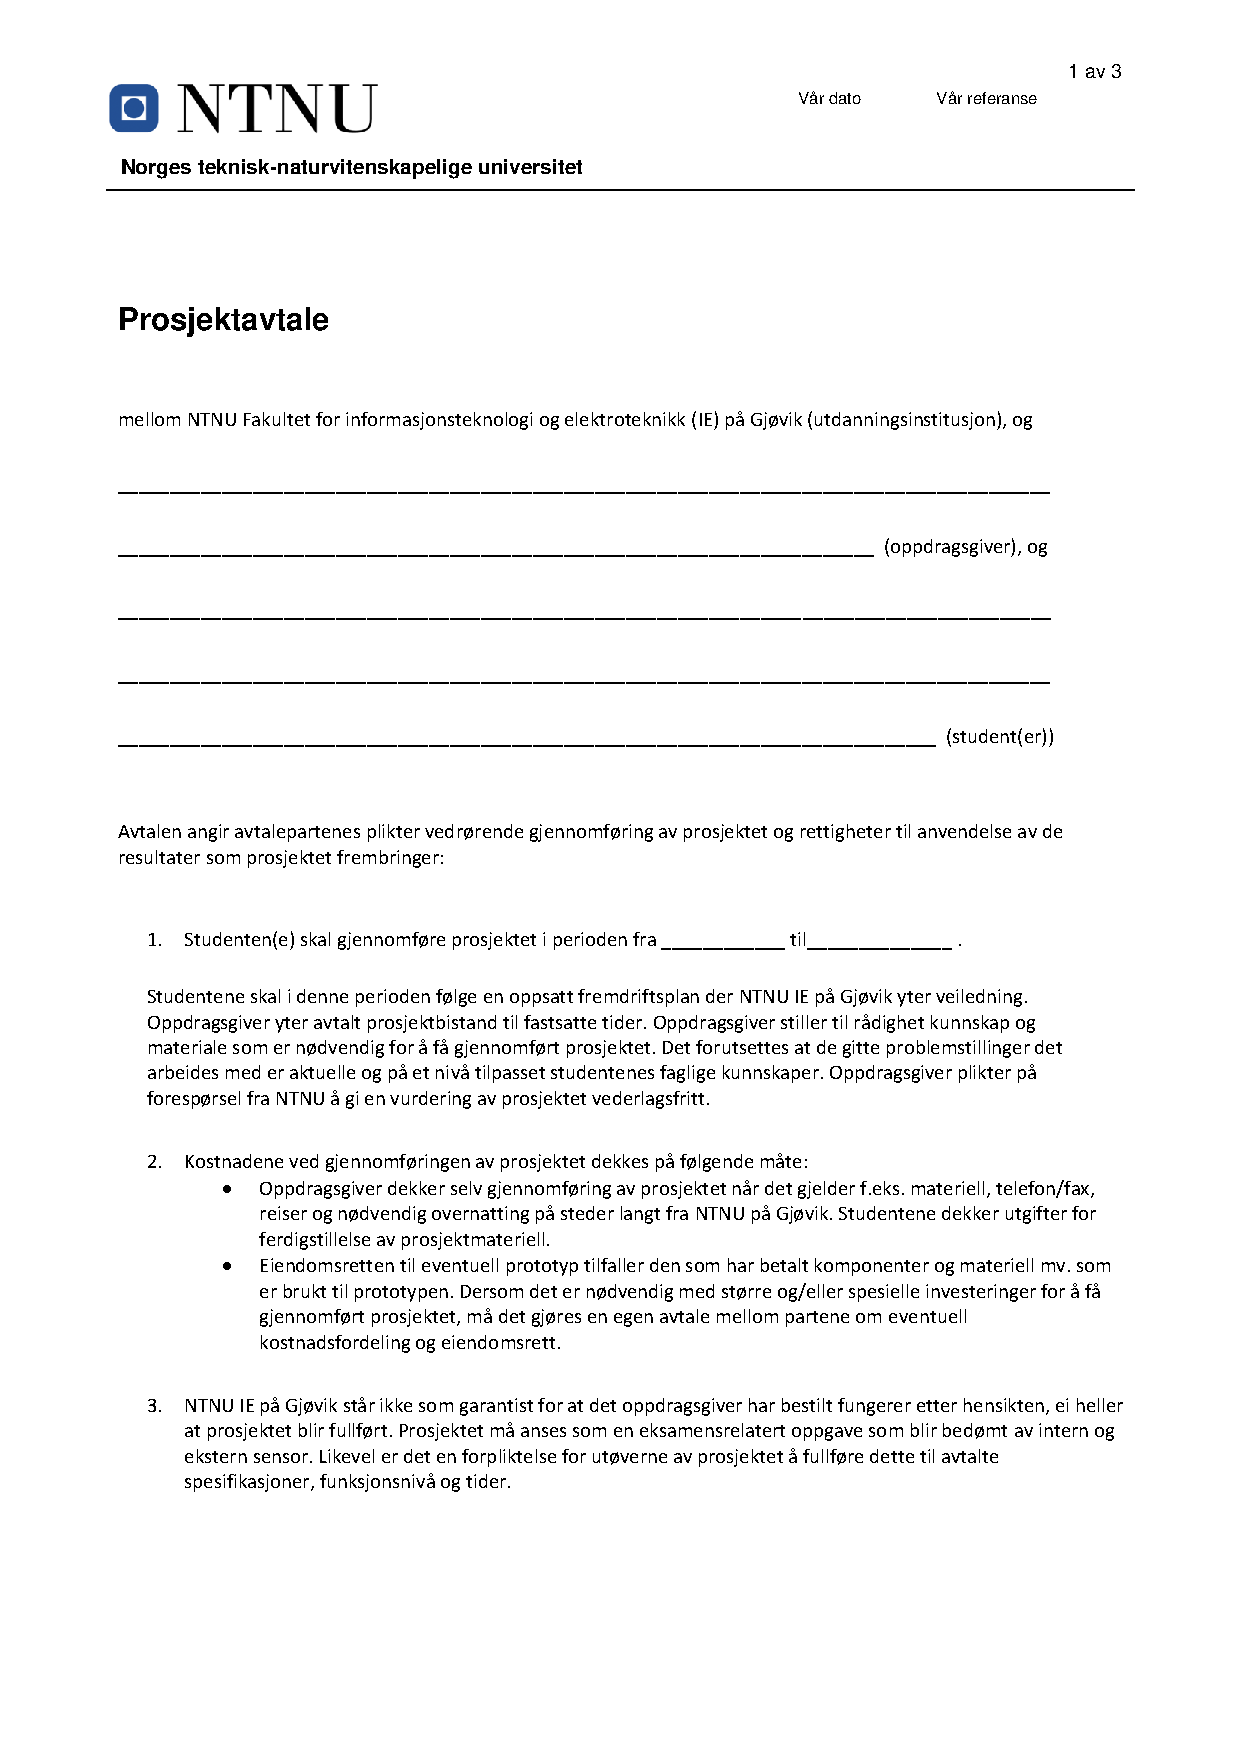
\includepdf[pages=-]{appendices/assets/NTNUProsjektavtale.pdf}

\end{document}
